% !Mode:: "TeX:UTF-8"
%%%%%%%%%%%%%%%%%%%%%%%%%%%%%%%%%%%%%%%%%%%%%%%%%%%%%%%%%%%%%%%%%%%%%%%%%%%%%%% 
%                          _
%  _____ ____ _ _ __  _ __| |___ ___
% / -_) \ / _` | '  \| '_ \ / -_|_-<
% \___/_\_\__,_|_|_|_| .__/_\___/__/
%                    |_|
%  _              _         _   _
% | |__ _  _   __| |_  _ __| |_(_)_ _  __ _  _ ___
% | '_ \ || | / _` | || (_-<  _| | ' \/ _| || (_-<
% |_.__/\_, | \__,_|\_,_/__/\__|_|_||_\__|\_, /__/
%       |__/                              |__/
%%%%%%%%%%%%%%%%%%%%%%%%%%%%%%%%%%%%%%%%%%%%%%%%%%%%%%%%%%%%%%%%%%%%%%%%%%%%%%%
\section{课题来源及研究的目的和意义}
\subsection{研究背景}
进入21世纪以来,多旋翼无人机领域取得了很大的发展。
为突破现在市场上主流的欠驱动无人机所存在的瓶颈,近年来人们又研制出了不少种的全驱动多旋翼无人机系统,
这种无人机可以跟踪6自由度轨迹,有效增强了多旋翼无人机的机动性能,拓宽了其应用场景。

作为一个高自由度且敏捷的系统,无人机的稳定自主飞行依赖鲁棒且高精度的导航系统来对自身和外界的状态进行有效估计。
同时定位与建图(Simultaneous Localization and Mapping, SLAM)技术\cite{liu2016asurvey}被广泛应用于移动机器人的实时定位导航中,
使得机器人在复杂的无GPS环境中也能获得准确的状态估计和环境感知。
其中,基于视觉或视觉惯性融合的SLAM导航技术(VSLAM或VISLAM)以其相对较低的成本、轻量级的硬件需求和较高的精度和鲁棒性成为适用于无人机的选择。

\subsection{研究的目的及意义}
% 视觉-惯性导航
移动机器人导航一直以来被广泛研究。
目前常用的导航方式是基于全球导航卫星系统(Global Navigation Satellite System, GNSS)的,
但是这种方法并不适用与室内、隧道等卫星信号质量差的环境。
SLAM技术则很好地弥补了基于GNSS的导航系统的局限性,
其具体是指搭载特定传感器的主体,在没有环境先验信息的情况下,于运动过程中建立环境的模型,同时估计自己的运动\cite{davison2007monoslam}。
可见传感器的选择是研究和实现SLAM技术的重点。

\begin{figure}[htbp]
    \centering
    \begin{minipage}{0.32\textwidth}
    \centering
    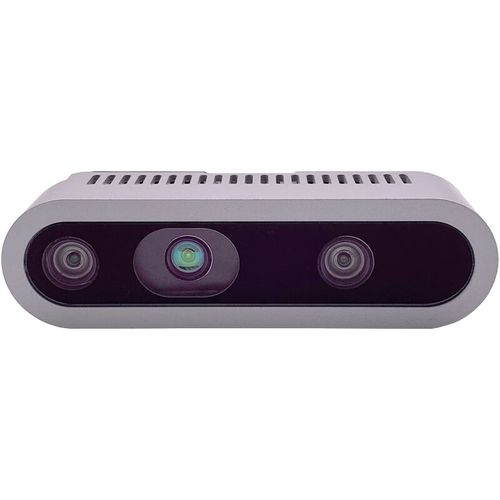
\includegraphics[width=\textwidth]{figures/visual_sensor.jpeg}
    \caption[subfig:rgbd_camera]{}{深度相机}
    \end{minipage}
    \centering
    \begin{minipage}{0.32\textwidth}
    \centering
    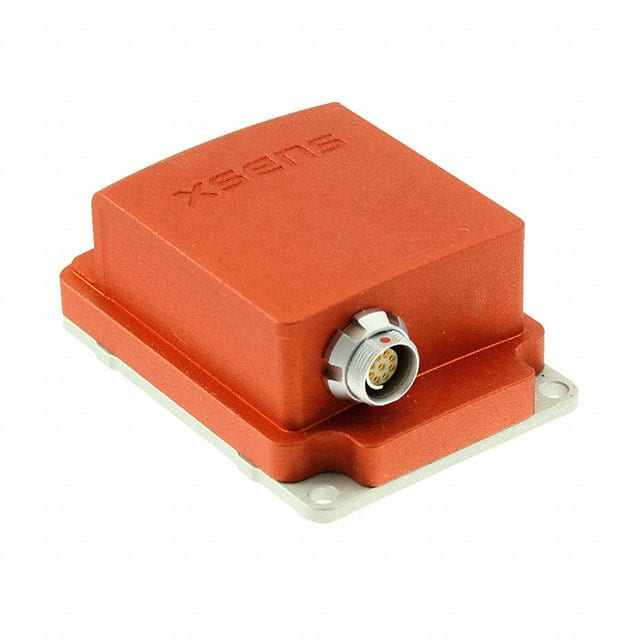
\includegraphics[width=\textwidth]{figures/inertial_sensor.jpeg}
    \caption[subfig:imu]{}{IMU}
    \end{minipage}
    \centering
    \begin{minipage}{0.32\textwidth}
    \centering
    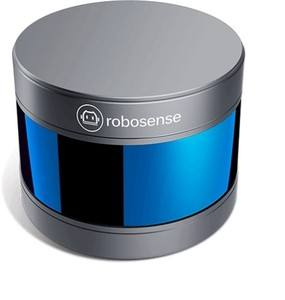
\includegraphics[width=\textwidth]{figures/lidar.jpeg}
    \caption[subfig:lidar]{}{激光雷达}
    \end{minipage}
    \caption{SLAM技术常用的传感器}
    \label{fig:common_sensors_for_slam}
\end{figure}

如图\ref{fig:common_sensors_for_slam}所示目前SLAM系统中常用的传感器有相机(视觉传感器)、惯性测量单元(Inertial Measurement Unit, IMU)和激光雷达等。
基于IMU的惯性导航是一项很经典的技术,并且已经发展得相当成熟,利用IMU提供的高频6DoF运动信息可以非常精确地估计姿态,
但是受IMU中陀螺仪和加速度计的零漂和噪声的影响,在积分求解位置的时候不可避免地会产生误差累积和漂移(drift),
因此,IMU一般不会单独用作SLAM的传感器。
基于激光雷达的SLAM导航技术也已经发展地比较成熟,但是激光雷达的体积和重量较大,而且成本较为高昂。
相对而言视觉传感器体积小、重量轻、成本低,并且能提供更为丰富的环境信息,这些特性使得视觉SLAM技术一直以来是学术界研究的热点。
然而视觉传感器同时也存在难以恢复尺度信息(主要针对于单目视觉)、低频、对光照敏感等问题。
实际上,在较为复杂的场景下仅靠单一的传感器是难以实现理想的导航定位效果的,
在这样的背景下,融合IMU和视觉信息的视觉-惯性导航系统(Visual-Inertial Navigation Systems, VINS)成为一个重要的研究课题。
VINS保留了纯视觉SLAM的小体量和低成本,并且结合了IMU和相机二者的优点,变得更加鲁棒和精确,在敏捷且追求轻量化的无人机系统上具有很高的研究价值和广阔的应用前景。

% 全驱动无人机
多旋翼无人机的驱动力包括3维的力$\bm{f} \in \mathbb{R}^3$和3维的力矩$\bm{\tau} \in \mathbb{R}^3$,
可将二者合并为一个6维向量$\bm{w} = \left[\bm{f}^\top \quad \bm{\tau}^\top\right]^\top \in \mathbb{R}^6$称为力旋量(wrench)。
产生驱动力的执行器指令对应控制输入$\bm{u} \in \mathbb{R}^{n_{\bm{u}}}$。
由力旋量$\bm{w_\text{act}}$求解对应控制输入$\bm{u}$的过程称为控制分配(control allocation),
如图\ref{fig:uav_classification}所示,我们按照控制分配雅可比(Jacobian)$\frac{\partial \bm{w_\text{act}}}{\partial \bm{u}}$的秩可将无人机分为欠驱动系统和全驱动系统\cite{bodie2022omnidirectional}。
目前常用的平行轴四旋翼、六旋翼等传统无人机属于欠驱动系统,它们的控制分配雅可比的秩为4,意味着它们只有4个控制自由度,
导致其机动性受限,且抗干扰能力弱。
为解决这些问题,充分发挥多旋翼飞行器的潜力,近年来发展出了多种全驱动无人机。
这些工作通过改变旋翼几何构型、增加旋翼倾转自由度等方式让旋翼能提供相对机身任意方向的推力和转矩,使得$\text{rank}(\frac{\partial \bm{w}_\text{act}}{\partial \bm{u}}) = 6$。
全驱动无人机能够独立地进行位置和姿态控制,具有任意姿态悬停、多旋翼飞行器跟踪6自由度全状态轨迹的能力,故又称为全向飞行器(omnidirectional aerial vehicle)。
进行这种受控的、自由的刚体运动是传统欠驱动多旋翼飞行器所无法做到的,这也赋予了全驱动无人机在空中作业、避障等方面具有很大的优势和潜力。

\begin{figure}[htbp]
    \centering
    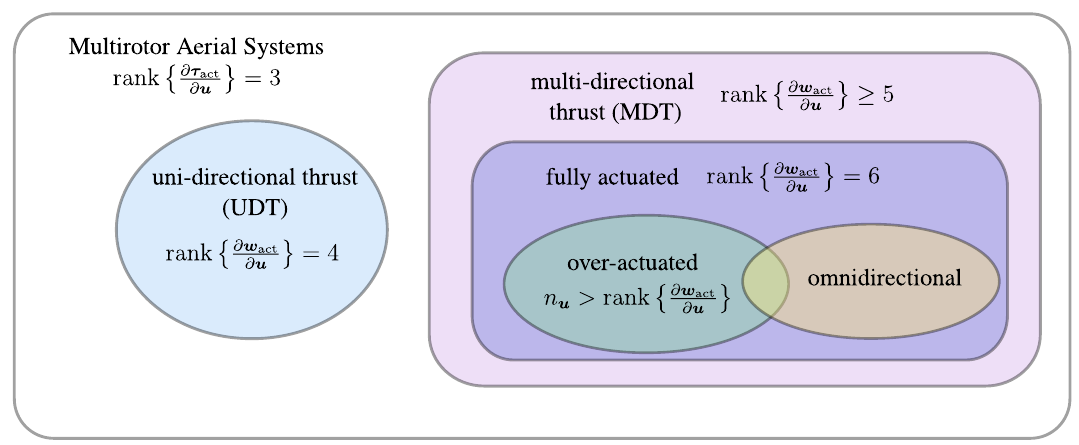
\includegraphics[width = \textwidth]{figures/uav_classification.png}
    \caption{无人机系统的分类\cite{bodie2022omnidirectional}}
    \label{fig:uav_classification}
\end{figure}

% 无人机外力估计
作用在无人机上的外部力旋量(external wrench)可以等效分解为作用在无人机质心上的外力(external force)和外力矩(external torque),
外力对无人机的平移动力学产生扰动,外力矩则对无人机的旋转动力学产生扰动,
这些扰动的来源可能有风扰、接触、机上载荷(如机械臂)以及空气动力学效应(如狭小空间中的乱流)等,
可能会严重影响无人机的正常作业。
为了补偿这些扰动,无人机的控制模块和规划模块需要精确地知晓外力和外力矩的大小和方向\cite{ding2021vid},
对于具有独立控制6自由度力和力矩能力的全驱动无人机而言,其具有比传统欠驱动无人机更优秀的扰动补偿能力。
因此,有必要为全驱动无人机设计一个显示考虑外部力旋量的状态估计器。

本课题的目标是设计一个基于视觉惯性融合的SLAM导航系统,
期望此系统能够:
\begin{enumerate}
    \item 精确且高效地估计自身运动;
    \item 能结合无人机的动力学模型精确且高效地估计外部作用力;
    \item 适用于全驱动无人机,并能结合建图与规划模块实现自主导航。
\end{enumerate}

\section{国内外研究现状及分析}
\subsection{国内外研究现状}
\subsubsection{视觉惯性导航研究现状}
\subsubsection{无人机的外力估计研究现状}
\subsubsection{全驱动旋翼无人机研究现状}
\subsection{国内外文献综述及简析}
\subsubsection{视觉惯性导航文献综述及简析}
\subsubsection{无人机的外力估计文献综述及简析}
\subsubsection{全驱动旋翼无人机文献综述及简析}
\section{前期的理论研究与试验论证工作的结果}
\section{学位论文的主要研究内容、实施方案及其可行性论证}
\subsection{主要研究内容}
(撰写宜使用将来时态,不能只列出论文目录来代替对研究内容的分析论述)
\subsection{实施方案及其可行性论证}
\section{论文进度安排,预期达到的目标}
\subsection{进度安排}
\subsection{预期达到的目标}
\section{学位论文预期创新点}
\section{为完成课题已具备和所需的条件、外协计划及经费}
\section{预计研究过程中可能遇到的困难、问题,以及解决的途径}
\section{主要参考文献}
\bibliographystyle{hitszthesis}
\bibliography{reference}

% Local Variables:
% TeX-master: "../report"
% TeX-engine: xetex
% End: